 \documentclass{beamer}
\mode<presentation>
\usepackage{amsmath}
\usepackage{amssymb}
%\usepackage{advdate}
\usepackage{graphicx}
\usepackage{adjustbox}
\usepackage{subcaption}
\usepackage{enumitem}
\usepackage{multicol}
\usepackage{mathtools}
\usepackage{listings}
\usepackage{url}
\def\UrlBreaks{\do\/\do-}
\usetheme{Boadilla}
\usecolortheme{lily}
\let\vec\mathbf
\setbeamertemplate{footline}
{
  \leavevmode%
  \hbox{%
  \begin{beamercolorbox}[wd=\paperwidth,ht=2.25ex,dp=1ex,right]{author in head/foot}%
    \insertframenumber{} / \inserttotalframenumber\hspace*{2ex} 
  \end{beamercolorbox}}%
  \vskip0pt%
}
\setbeamertemplate{navigation symbols}{}

\providecommand{\nCr}[2]{\,^{#1}C_{#2}} % nCr
\providecommand{\nPr}[2]{\,^{#1}P_{#2}} % nPr
\providecommand{\mbf}{\mathbf}
\providecommand{\pr}[1]{\ensuremath{\Pr\left(#1\right)}}
\providecommand{\qfunc}[1]{\ensuremath{Q\left(#1\right)}}
\providecommand{\sbrak}[1]{\ensuremath{{}\left[#1\right]}}
\providecommand{\lsbrak}[1]{\ensuremath{{}\left[#1\right.}}
\providecommand{\rsbrak}[1]{\ensuremath{{}\left.#1\right]}}
\providecommand{\brak}[1]{\ensuremath{\left(#1\right)}}
\providecommand{\lbrak}[1]{\ensuremath{\left(#1\right.}}
\providecommand{\rbrak}[1]{\ensuremath{\left.#1\right)}}
\providecommand{\cbrak}[1]{\ensuremath{\left\{#1\right\}}}
\providecommand{\lcbrak}[1]{\ensuremath{\left\{#1\right.}}
\providecommand{\rcbrak}[1]{\ensuremath{\left.#1\right\}}}
\theoremstyle{remark}
\newtheorem{rem}{Remark}
\newcommand{\sgn}{\mathop{\mathrm{sgn}}}
\providecommand{\abs}[1]{\vert#1\vert}
\providecommand{\res}[1]{\Res\displaylimits_{#1}} 
\providecommand{\norm}[1]{\lVert#1\rVert}
\providecommand{\mtx}[1]{\mathbf{#1}}
\providecommand{\mean}[1]{E[ #1 ]}
\providecommand{\fourier}{\overset{\mathcal{F}}{ \rightleftharpoons}}
%\providecommand{\hilbert}{\overset{\mathcal{H}}{ \rightleftharpoons}}
\providecommand{\system}[1]{\overset{\mathcal{#1}}{ \longleftrightarrow}}
%\providecommand{\system}{\overset{\mathcal{H}}{ \longleftrightarrow}}
	%\newcommand{\solution}[2]{\vec{Solution:}{#1}}
%\newcommand{\solution}{\noindent \vec{Solution: }}
\providecommand{\dec}[2]{\ensuremath{\overset{#1}{\underset{#2}{\gtrless}}}}
\newcommand{\myvec}[1]{\ensuremath{\begin{pmatrix}#1\end{pmatrix}}}


\lstset{
%language=C,
frame=single, 
breaklines=true,
columns=fullflexible
}
\lstset{
  language=C,
  basicstyle=\ttfamily\footnotesize,
  keywordstyle=\color{blue}\bfseries,
  commentstyle=\color{gray}\itshape,
  stringstyle=\color{orange},
  numbers=left,
  numberstyle=\tiny\color{gray},
  breaklines=true,
  frame=single,
  showstringspaces=false,
  tabsize=4,
  captionpos=b
}
\numberwithin{equation}{section}
\lstset{
  language=Python,
  basicstyle=\ttfamily\small,
  keywordstyle=\color{blue},
  stringstyle=\color{orange},
  numbers=left,
  numberstyle=\tiny\color{gray},
  breaklines=true,
  showstringspaces=false
}

\title{Problem 12.9}
\author{Sujal Rajani}

\date{\today} 
\begin{document}

\begin{frame}
\titlepage
\end{frame}

\section{Question}
\begin{frame}{Question}
\textbf{Question }:
given the wavelet , a=\{3,-2\} and b=\{1,-2\},the cross-correlation , $\phi_{ab}$,is given by .
\end{frame}
\begin{frame}{Solution}
\textbf{SOLUTION}
Given the sequences
\begin{align*}
\vec{a} = \myvec{3\\-2}, \vec{ b} = \myvec{1\\-2}.
\end{align*}
The cross-correlation between $a[n]$ and $b[n]$ is defined as
\[
\phi_{ab}[k] = \sum_{n} a[n]\, b[n+k].
\]
For sequences of length $2$, the cross-correlation length is
\[
L = 2+2-1 = 3, \quad k = -1, 0, 1.
\]
     \end{frame}
     \begin{frame}{Frame Title}
       \subsection*{Matrix Representation}

The cross-correlation can be represented as a matrix multiplication:
\[
\boldsymbol{{\phi}_{ab}}=
\myvec{
\phi_{ab}[-1] \\[0.4em]
\phi_{ab}[0] \\[0.4em]
\phi_{ab}[1]
}
\]

\noindent
This matrix corresponds to the shifted overlaps between $a[n]$ and $b[n]$:

\begin{itemize}
    \item First row $\rightarrow$ shift $-1$ (overlap with $b[1]$)
    \item Second row $\rightarrow$ shift $0$ (full overlap)
    \item Third row $\rightarrow$ shift $+1$ (overlap with $b[0]$)
\end{itemize}

     \end{frame}
     \begin{frame}{ Step-by-Step Calculation}    
\[
\begin{aligned}
\phi_{ab}[-1] &= a[0]\,b[1] = 3 \times (-2) = -6, \\
\phi_{ab}[0]  &= a[0]\,b[0] + a[1]\,b[1] = 3\times 1 + (-2)\times (-2) = 3 + 4 = 7, \\
\phi_{ab}[1]  &= a[1]\,b[0] = (-2)\times 1 = -2.
\end{aligned}
\]

\subsection*{Final Answer}

\[
\boldsymbol{{\phi}_{ab}}=
\myvec{
\phi_{ab}[-1]\\[0.4em]
\phi_{ab}[0]\\[0.4em]
\phi_{ab}[1]
}
=
\myvec{
-6\\[0.4em]
7\\[0.4em]
-2
}.
\]

\[
\boxed{\phi_{ab}[k] = \{-6,\ 7,\ -2\}}
\] 
     \end{frame}
       \begin{frame}[fragile]
    \begin{figure}[H]
    \centering
    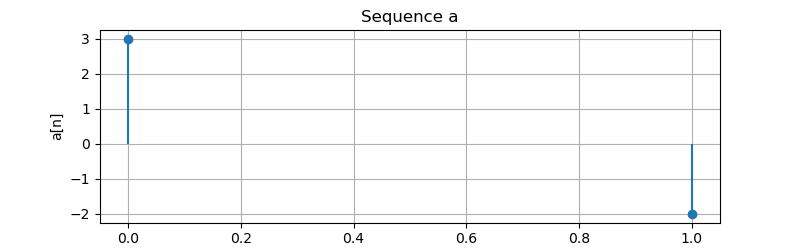
\includegraphics[width = 0.6\columnwidth]{../figs/img1.png}
    \caption*{}
    \label{figs}
\end{figure}
\end{frame}
  \begin{frame}[fragile]
    \begin{figure}[H]
    \centering
    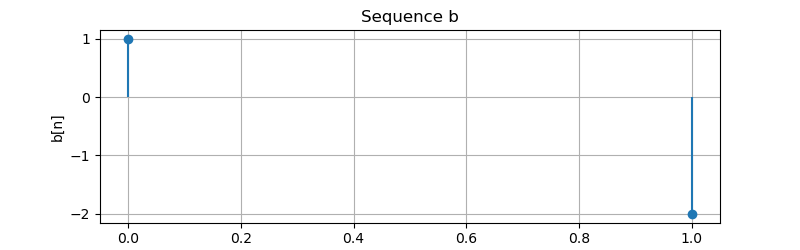
\includegraphics[width = 0.6\columnwidth]{../figs/img2.png}
    \caption*{}
    \label{figs}
\end{figure}
\end{frame}
  \begin{frame}[fragile]
    \begin{figure}[H]
    \centering
    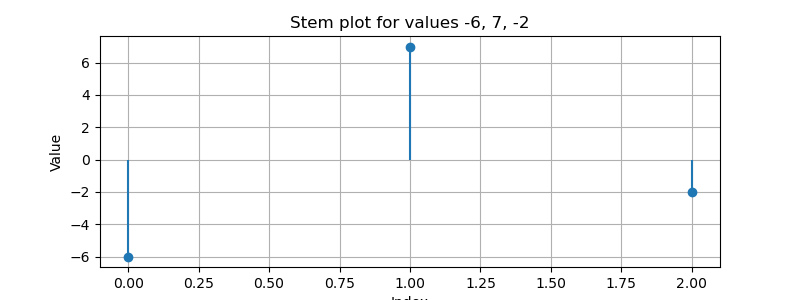
\includegraphics[width = 0.6\columnwidth]{../figs/img3.png}
    \caption*{}
    \label{figs}
\end{figure}
\end{frame}
\end{document}